\documentclass[12pt,a4paper]{report}
\usepackage[T2A]{fontenc}
\usepackage[utf8]{inputenc}
\usepackage[russian]{babel}
\usepackage{graphicx, setspace, amsmath, amsfonts}

\usepackage[
top = 1.25cm, 
bottom = 2.0cm]{geometry}

\begin{document}
\begin{titlepage} 
	\centering
    % HEADER
	{
        \scshape
        Федеральное государственное автономное образовательное учреждение высшего образования
        \par
        \textbf{«Научно-образовательная корпорация ИТМО»}
        \par
        \vspace*{1cm}
        Факультет Программной Инженерии и Компьютерной Техники
        \par
    }
    % LOGO
    \vspace*{0.6cm}
    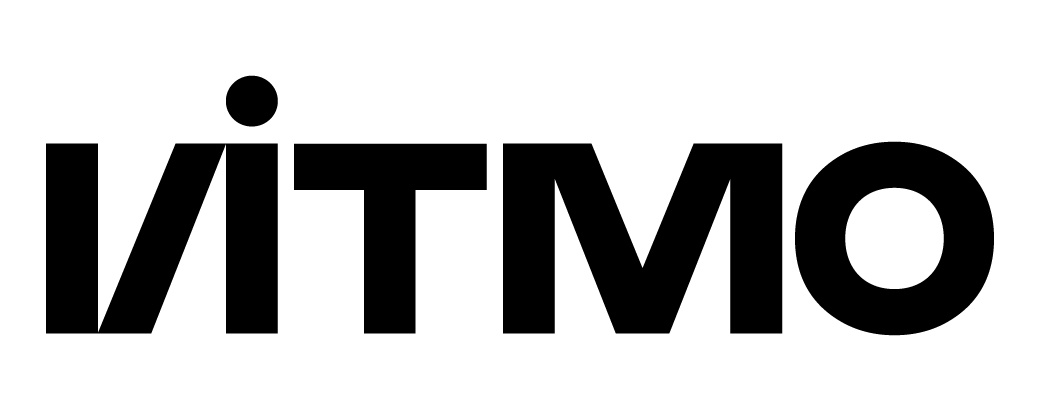
\includegraphics[width=\textwidth]{logo.png}
    % LAB INFO
    {
        \Large
        \textbf{Домашнее задание по теории графов №6}
        \par
        \normalsize
        \vspace*{0.75cm}
        \textbf{Вариант 92}
        \par
    }
    \vfill
    % СREDITS
    \hfill\begin{minipage}{\dimexpr\textwidth-7.8cm}
        \textbf{Выполнил:}\par
        Степанов Арсений Алексеевич\par
        \vspace*{0.15cm}
        \textbf{Группа:}\par
        P3109\par
        \vspace*{0.15cm}
        \textbf{Преподаватель:}\par
        Поляков Владимир Иванович\par
    \end{minipage}
    \vfill
    Санкт-Петербург, \the\year{}г.
\end{titlepage}   
\onehalfspacing
\section*{Матрица смежности графа}
Тк у исходного графа нечётное кол-во связей у вершин $e_1$, $e_2$, $e_6$, $e_7$, $e_9$ и $e_{10}$ нечётное, соединим $e_1$ и $e_2$ и разъеденим $e_6$ и $e_7$, $e_9$ и $e_{10}$, для того чтобы граф содержал эйлеров цикл \\
\hfill\break
\begin{tabular}{|c|c|c|c|c|c|c|c|c|c|c|c|c|c|}
    \hline
    V/V & $e_{1}$ & $e_{2}$ & $e_{3}$ & $e_{4}$ & $e_{5}$ & $e_{6}$ & $e_{7}$ & $e_{8}$ & $e_{9}$ & $e_{10}$ & $e_{11}$ & $e_{12}$ \\
    \hline
    $e_{1}$  & 0 & 1 &   & 1 &   &   &   & 1 & 1 & 1 &   & 1 \\
    \hline
    $e_{2}$  & 1 & 0 &   &   & 1 &   & 1 &   & 1 &   &   &   \\
    \hline
    $e_{3}$  &   &   & 0 & 1 &   & 1 & 1 & 1 &   & 1 & 1 &   \\
    \hline
    $e_{4}$  & 1 &   & 1 & 0 &   &   & 1 &   &   &   &   & 1 \\
    \hline
    $e_{1}$  &   & 1 &   &   & 0 & 1 & 1 &   &   &   &   & 1 \\
    \hline
    $e_{6}$  &   &   & 1 &   & 1 & 0 &   &   & 1 &   &   & 1 \\
    \hline
    $e_{7}$  &   & 1 & 1 & 1 & 1 &   & 0 & 1 &   &   & 1 &   \\
    \hline
    $e_{8}$  & 1 &   & 1 &   &   &   & 1 & 0 &   &   & 1 &   \\
    \hline
    $e_{9}$  & 1 & 1 &   &   &   & 1 &   &   & 0 &   & 1 &   \\
    \hline
    $e_{10}$ & 1 &   & 1 &   &   &   &   &   &   & 0 & 1 & 1 \\
    \hline
    $e_{11}$ &   &   & 1 &   &   &   & 1 & 1 & 1 & 1 & 0 & 1 \\
    \hline
    $e_{12}$ & 1 &   &   & 1 & 1 & 1 &   &   &   & 1 & 1 & 0 \\
    \hline
\end{tabular}
\section*{Нахождение цикла}
Возьмём вершину $e_{1}$ \\
Выбирем ребро $e_{1-2}$ \\
Возьмём вершину $e_{2}$ \\
Выбирем ребро $e_{2-5}$ \\
Возьмём вершину $e_{5}$ \\
Выбирем ребро $e_{5-6}$ \\
Возьмём вершину $e_{6}$ \\
Выбирем ребро $e_{6-3}$ \\
Возьмём вершину $e_{3}$ \\
Выбирем ребро $e_{3-4}$ \\
Возьмём вершину $e_{4}$ \\
Выбирем ребро $e_{4-1}$ \\
Возьмём вершину $e_{1}$ \\
Выбирем ребро $e_{1-8}$ \\
Возьмём вершину $e_{8}$ \\
Выбирем ребро $e_{8-3}$ \\
Возьмём вершину $e_{3}$ \\
Выбирем ребро $e_{3-7}$ \\
Возьмём вершину $e_{7}$ \\
Выбирем ребро $e_{7-2}$ \\
Возьмём вершину $e_{2}$ \\
Выбирем ребро $e_{2-9}$ \\
Возьмём вершину $e_{9}$ \\
Выбирем ребро $e_{9-1}$ \\
Возьмём вершину $e_{1}$ \\
Выбирем ребро $e_{1-10}$ \\
Возьмём вершину $e_{10}$ \\
Выбирем ребро $e_{10-3}$ \\
Возьмём вершину $e_{3}$ \\
Выбирем ребро $e_{3-11}$ \\
Возьмём вершину $e_{11}$ \\
Выбирем ребро $e_{11-7}$ \\
Возьмём вершину $e_{7}$ \\
Выбирем ребро $e_{7-4}$ \\
Возьмём вершину $e_{4}$ \\
Выбирем ребро $e_{4-12}$ \\
Возьмём вершину $e_{12}$ \\
Выбирем ребро $e_{12-5}$ \\
Возьмём вершину $e_{5}$ \\
Выбирем ребро $e_{5-7}$ \\
Возьмём вершину $e_{7}$ \\
Выбирем ребро $e_{7-8}$ \\
Возьмём вершину $e_{8}$ \\ 
Выбирем ребро $e_{8-11}$ \\
Возьмём вершину $e_{11}$ \\ 
Выбирем ребро $e_{11-9}$ \\
Возьмём вершину $e_{9}$ \\
Выбирем ребро $e_{9-6}$ \\ 
Возьмём вершину $e_{6}$ \\
Выбирем ребро $e_{6-12}$ \\
Возьмём вершину $e_{12}$ \\
Выбирем ребро $e_{12-10}$ \\
Возьмём вершину $e_{10}$ \\
Выбирем ребро $e_{10-11}$ \\
Возьмём вершину $e_{11}$ \\
Выбирем ребро $e_{11-12}$ \\
Возьмём вершину $e_{12}$ \\ 
Выбирем ребро $e_{12-1}$ \\
\hfill\break
\\
\\
\\
Эйлеров цикл получен:\\
$e_{1} \rightarrow e_{2}\rightarrow e_{5}\rightarrow e_{6}\rightarrow e_{3}\rightarrow e_{4}\rightarrow e_{1}\rightarrow e_{8}\rightarrow e_{3}\rightarrow e_{7}\rightarrow e_{2}\rightarrow e_{9}\rightarrow e_{1}\rightarrow e_{10}\rightarrow e_{3}\rightarrow e_{11}\rightarrow e_{7}\rightarrow e_{4}\rightarrow e_{12}\rightarrow e_{5}\rightarrow e_{7}\rightarrow e_{8}\rightarrow e_{11}\rightarrow e_{9}\rightarrow e_{6}\rightarrow e_{12}\rightarrow e_{10}\rightarrow e_{11}\rightarrow e_{12}\rightarrow e_{1}$
\end{document}
